\documentclass[answers,addpoints,12pt]{exam}
\usepackage{multicol,xy}
\usepackage{graphicx,multicol}
\usepackage[euler-digits]{eulervm}
\usepackage{charter,amsmath,amssymb}
\usepackage[letterpaper,margin=1in]{geometry}
\pagestyle{headandfoot}
\runningheadrule
\firstpageheader{\bf Math 104}{\bf Exam 2, Red Form}{\bf 8 October 2014}
\runningheader{\bf Math 104}
{\bf Exam Two, Page \thepage\ of \numpages}
{\bf 8 October 2014}
\firstpagefooter{}{}{}
\runningfooter{}{}{}
\everymath{\displaystyle}
\begin{document}

\begin{center}
\fbox{\fbox{\parbox{5.5in}{
This exam has \numquestions~questions.
It has been printed on \numpages~pages and is worth \numpoints~points.
Answer all the questions below in the spaces provided.
In order to receive maximum credit, you must
clearly indicate how you arrived at your answers.
By signing below, you pledge that you
\begin{enumerate}
\item will not communicate to any person in any conceivable way anything
about the contents of this exam
until all students have taken the exam, and
\item in taking this exam now,
you have not been the recipient of such communication from anyone else.
\end{enumerate}}}}
\end{center}
\vspace{.2in}
\makebox[\textwidth]{Your signature:\enspace\hrulefill}\\
\vspace{.2in}\\
\makebox[\textwidth]{Your name:\enspace\hrulefill}\\
\vspace{.2in}\\
\makebox[\textwidth]{Your student ID number:\enspace\hrulefill}\\

\begin{questions}

\question[16] Two dice are rolled and the
numbers showing on the top faces are observed.
Determine the odds against each of the following events.
\begin{parts}
\part Both numbers are the same
\vspace{.25in}
\part The sum of the two numbers is $5$
\vspace{.25in}
\part The sum of the two numbers is even
\vspace{.25in}
\part At least one of the numbers is $3$
\end{parts}
\begin{solution}
\begin{parts}
\part Can occur in $6$ ways, so $30:6$ or $5:1$ the odds against
\part Can occur in $4$ ways, so $32:4$ or $8:1$ the odds against
\part Can occur in $18$ ways, so $18:18$ or $1:1$ the odds against
\part Can occur in $11$ ways, so $25:11$ the odds against
\end{parts}
\end{solution}

\question[10]
\begin{multicols}{2}
If you drop a thumbtack on the floor, it either lands point down
or point up, as shown in the image at the right.
You drop all the thumbtacks in a box on the floor, observing that
$105$~tacks land point down while $35$ land point up.
Based on these results, if you drop two thumbtacks on the floor, what
is the probability that both tacks will land point up?
\columnbreak\\
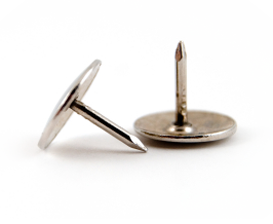
\includegraphics[scale=.6]{Thumbtacks}
\end{multicols}
\begin{solution}
$\frac{35}{35+105}=\frac{1}{4}$ the empirical probability
of point up, so $\left(\frac{1}{4}\right)^2=\frac{1}{16}$
the probability of both points up.
\end{solution}

\question[10] A game is played as follows.
Two coins are flipped. If both coins come up
heads, then you win $\$2$. If both coins come
up tails, then you win $\$3$. 
Otherwise you lose $\$4$. What are your expected proceeds
of this game?
\begin{solution}
$2\left(\frac{1}{4}\right)+3\left(\frac{1}{4}\right)
-4\left(\frac{1}{2}\right)=-\frac{3}{4}=\$-0.75$
\end{solution}

\question[15] Suppose $E$ and $F$ are events
and $P\left(E\right)=0.75$ and $P\left(F\right)=0.25$.
\begin{parts}
\part Calculate $P\left(\text{$E$ or $F$}\right)$
assuming that $E$ and $F$ are mutually exclusive.
\part Calculate $P\left(\text{$E$ and $F$}\right)$
assuming $E$ and $F$ are independent.
\part Calculate $P\left(\text{$E$ or $F$}\right)$
assuming $E$ and $F$ are independent.
\end{parts}
\begin{solution}
\begin{parts}
\part $0.75+0.25=1.0$
\part $0.75\cdot 0.25=0.1875$
\part $0.75+0.25-0.1875=0.8125$
\end{parts}
\end{solution}

\question[12] Ames High School has $1422$ students.
$102$ students are in band but not chorus while
$176$ students are in chorus but not band.
If $1093$ students are in neither band nor chorus,
then how many students are in both band and chorus?
\begin{solution}
\[\begin{xy}<.5cm,0cm>:
(-1,2)*+!D{\text{B}};
(1,2)*+!D{\text{C}};
(-1,0)*\cir<1cm>{};
(1,0)*\cir<1cm>{};
(0,0)*{51};
(-2,0)*{102};
(2,0)*{176};
(4,0)*{1093};
\end{xy}\]
\end{solution}

\question[15] Your itinerary for Saturday should
include a trip to Target, Staples, Hy-Vee, and the bank.
However, since Target is across the street from Staples,
you should visit those two stores consecutively. In other
words, you should visit Target right after Staples, or else
Staples right after Target. In how many ways
can you plan your itinerary?
\begin{solution}12\end{solution}

\question[10] If two cards are randomly selected from a deck
of playing cards without replacement, what is the probability that both cards
will be picture cards?  A {\em picture card} is either a Jack, Queen, or King.
\begin{solution}
$\frac{12}{52}\cdot\frac{11}{51}=\frac{11}{121}\approx 0.0498$
\end{solution}

\question[12] A Math~104 quiz has ten multiple-choice
questions, each with five answer choices. If you guess on all
ten questions, what is the probability that you will answer at
least one question correctly?
\begin{solution}
$1-\left(\frac{4}{5}\right)^{10}\approx 0.8926$
\end{solution}

\end{questions}

\vfill
\begin{center}\gradetable[h][questions]\end{center}

\end{document}
